% Preliminaries
\chapter{Preliminaries}\label{preliminaries}
	Before we define our specific data models and problems we will introduce and formalize commonly reoccurring terms.

% Graph
\section{Graph}
	\begin{mydef}\label{graph}
		A \textnormal{graph} $G$ is a tuple $(V, E)$ with a set of nodes $V$ and a set of
		edges $E \subseteq V \times \mathbb{R}_{\ge 0} \times V$.
		An \textnormal{edge} $e \in E$ is an ordered tuple $(u, w, v)$ with a source node $u \in V$, a non-negative
		weight $w \in \mathbb{R}_{\ge 0}$ and a destination node $v \in V$.
	\end{mydef}\quad\\
	Note that \defref{graph} actually defines a \textit{directed} graph, as opposed to an \textit{undirected} graph where an
	edge like $(u, w, v)$ would be considered equal to the edge of opposite direction $(v, w, u)$ (compare to \libref{graphTheory}).
	However, for transportation networks an undirected graph often is not applicable, for example, due to one way streets or
	time dependent connections like trains which depart at different times for different directions.
	
	In the context of route planning we refer to the weight $w$ of an edge $(u, w, v)$ as \textit{cost}. It can be used to encode the length
	of the represented connection. Or to represent the time it takes to travel the distance in a given
	transportation mode.
	% Graph example
	\begin{figure}[!ht]
		\begin{center}
			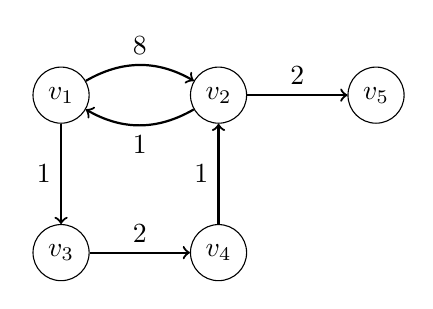
\begin{tikzpicture}[y = -1cm]
			 	% Nodes
			 	\node[circle, draw] (v1) at (0, 0) {$v_1$};
			 	\node[circle, draw] (v2) at (2, 0) {$v_2$};
			 	\node[circle, draw] (v3) at (0, 2) {$v_3$};
			 	\node[circle, draw] (v4) at (2, 2) {$v_4$};
			 	\node[circle, draw] (v5) at (4, 0) {$v_5$};
			 	
			 	% Edges
			 	\draw[thick, ->] (v1) to [bend left] node[above] {$8$} (v2);
			 	\draw[thick, ->] (v2) to node[above] {$2$} (v5);
			 	\draw[thick, ->] (v2) to [bend left] node[below] {$1$} (v1);
			 	\draw[thick, ->] (v1) to node[left] {$1$} (v3);
			 	\draw[thick, ->] (v3) to node[above] {$2$} (v4);
			 	\draw[thick, ->] (v4) to node[left] {$1$} (v2);
			\end{tikzpicture}
		\end{center}
		\caption{Illustration of an example graph with five nodes and six edges.}
		\label{graph_example}
	\end{figure}\quad\\
	As an example, consider the graph $G = (V, E)$ with
	\begin{align*}
		V	&= \{v_1, v_2, v_3, v_4, v_5\} \text{ and}\\
		E	&= \{(v_1, 8, v_2), (v_1, 1, v_3), (v_2, 1, v_1), (v_2, 2, v_5), (v_3, 2, v_4), (v_4, 1, v_2)\},
	\end{align*}
	which is illustrated in \figref{graph_example}.
	\begin{mydef}
		Given a graph $G = (V, E)$ the function $\src: E \to V, (u, w, v) \mapsto u$ gets the \textnormal{source}
		of an edge. Analogously $\dest: E \to V, (u, w, v) \mapsto v$ retrieves the \textnormal{destination}.
	\end{mydef}
	\begin{mydef}\label{path}
		A \textnormal{path} in a graph $G = (V, E)$ is a sequence $p = e_1e_2e_3\ldots$ of edges $e_i \in E$ such that
		\begin{align*}
			\forall i: \dest(e_i) = \src(e_{i + 1}).
		\end{align*}
		We write $e \in p$ if an edge $e$ appears at least once in the path $p$.
		The \textnormal{length} of a path is the amount of edges it contains, i.e. the length of the sequence.
		The \textnormal{weight} or \textnormal{cost} is the sum of its edges weights.
		
		Let $k$ be the length of a path $p$, then we define:
		\begin{align*}
			\src(p)	&= \src(e_1)\\
			\dest(p)	&= \dest(e_k)
		\end{align*}\quad\\
		Given two paths $q_1 = e_1\ldots e_k$ and $q_2 = e'_1\ldots e'_l$ where $\dest(e_k) = \src(e'_1)$,
		the concatenation of both paths is a path
		\begin{align*}
			p	&= e_1\ldots e_k e'_1\ldots e'_l
		\end{align*}
		with length $k + l$, also denoted by $p = q_1q_2$.
	\end{mydef}\quad\\
	An example of a path in the graph $G$ would be
	\begin{align*}
		p	&=(v_1, 8, v_2)(v_2, 1, v_1)(v_1, 1, v_3).
	\end{align*}
	Its length is $3$ and it has a weight of $10$.
	
% Tree
\section{Tree}
	\begin{mydef}\label{tree}
		A \textnormal{tree} is a graph $T = (V, E)$ with the following properties:
		\begin{itemize}
			\item[1.] There is exactly one node $r \in V$ with no ingoing edges, called the \textnormal{root}, i.e.
				\begin{align*}
					\exists! r \in V \nexists e \in E : \dest(e) = r.
				\end{align*}
			\item[2.] All other nodes $v$ have exactly one ingoing edge. The source $p$ of this edge is called \textnormal{parent} of $v$ and
				$v$ is called \textnormal{child} of $p$:
				\begin{align*}
					\forall v \in V : v \neq r \Rightarrow \exists! e \in E : \dest(e) = v.
				\end{align*}
		\end{itemize}
	\end{mydef}
	\begin{mydef}\label{subTree}
		The \textnormal{subtree} of a tree $T = (V, E)$ rooted at a node $r' \in V$ is a tree $T' = (V', E')$. $V' \subseteq V$ is the set
		of nodes that can be reached from $r'$. That is, all nodes that are part of possible paths starting at $r'$.
		Likewise, $E' \subseteq E$ is the set of edges restricted to the vertices in $V'$. The root of $T'$ is $r'$.
	\end{mydef}
	\begin{mydef}\label{treeDepth}
		The \textnormal{depth} of a node $v$ in a tree $T = (V, E)$, denoted by $\depth(v)$, is defined as the amount of
		edges between $v$ and the root $r$. It is the length of the unique path $p$ starting at $r$ and ending at $v$.
		
		The \textnormal{height} of a tree is its greatest depth, i.e.
		\begin{align*}
			\max_{v \in V} \depth(v).
		\end{align*}
		And
		\begin{align*}
			\children(v)	&= \{c \in T | c \text{ child of } v\}.
		\end{align*}
	\end{mydef}\quad\\
	Trees are hierarchical data-structures. Every node, except the root, has one parent. A node itself can have multiple children.
	Note that it is not possible to form a loop in a tree, i.e. a path that visits a node more than once. A node without
	children is called a \textit{leaf}.\\
	% Tree example
	\begin{figure}[!ht]
		\begin{center}
			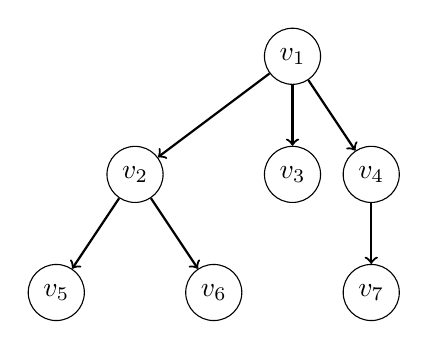
\begin{tikzpicture}[y = -1cm]
			 	% Nodes
			 	\node[circle, draw] (v1) at (3, 0) {$v_1$};
			 	\node[circle, draw] (v2) at (1, 1.5) {$v_2$};
			 	\node[circle, draw] (v3) at (3, 1.5) {$v_3$};
			 	\node[circle, draw] (v4) at (4, 1.5) {$v_4$};
			 	\node[circle, draw] (v5) at (0, 3) {$v_5$};
			 	\node[circle, draw] (v6) at (2, 3) {$v_6$};
			 	\node[circle, draw] (v7) at (4, 3) {$v_7$};
			 	
			 	% Edges
			 	\draw[thick, ->] (v1) to (v2);
			 	\draw[thick, ->] (v1) to (v3);
			 	\draw[thick, ->] (v1) to (v4);
			 	\draw[thick, ->] (v2) to (v5);
			 	\draw[thick, ->] (v2) to (v6);
			 	\draw[thick, ->] (v4) to (v7);
			\end{tikzpicture}\qquad\qquad\qquad
			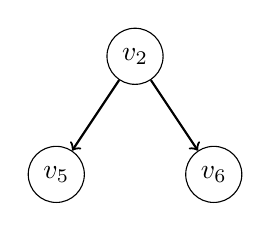
\begin{tikzpicture}[y = -1cm]
			 	% Nodes
			 	\node[circle, draw] (v2) at (1, 0) {$v_2$};
			 	\node[circle, draw] (v5) at (0, 1.5) {$v_5$};
			 	\node[circle, draw] (v6) at (2, 1.5) {$v_6$};
			 	
			 	% Edges
			 	\draw[thick, ->] (v2) to (v5);
			 	\draw[thick, ->] (v2) to (v6);
			\end{tikzpicture}
		\end{center}
		\caption{An example of an unlabeled tree (left) and the subtree of $v_2$ (right).}
		\label{treeExample}
	\end{figure}\quad\\
	\figref{treeExample} shows a tree with $7$ nodes. The node $v_1$ is the root; $v_5, v_6, v_3$
	and $v_7$ are the leaves. The tree has a height of $2$, the depth of $v_4$ is $1$. The subtree rooted at $v_2$
	only consists of the nodes $v_2, v_5$ and $v_6$.

% Automaton
\section{Automaton}\label{automaton_sec}
	Automata are labeled graphs. They are used to represent states and the correlation between them.
	\begin{mydef}\label{automaton}
		A \textnormal{deterministic finite automaton} (\dfa) $A$ is a tuple $(Q, \sigma, \Delta, q_0, F)$ with
		\begin{itemize}
			\item a set of states $Q$,
			\item a set of labels $\sigma$, called \textnormal{alphabet},
			\item a transition relation $\Delta \subseteq Q \times \sigma \times Q$,
			\item an initial state $q_0 \in Q$ and
			\item a set of accepting states $F \subseteq Q$.
		\end{itemize}
	\end{mydef}
	\begin{mydef}
		A \textnormal{word} $w \in \Sigma^{\star}$ is a finite sequence of letters
		\begin{align*}
			w	&= a_0a_1a_2 \ldots a_{k - 1}
		\end{align*}
		with $a_i \in \Sigma$ and some $k \in \mathbb{N}$. The empty word is denoted by $\varepsilon$.
		
		A word is called \textnormal{accepted} iff
		\begin{itemize}
			\item[1.] \begin{align*}
					\forall i: (q_i, a_i, q_{i + 1}) \in \Delta,
				\end{align*}
				for some $q_i \in Q$,
			\item[2.] $q_0$ is the initial state of the automaton and
			\item[3.] the last state is accepting, i.e. $q_k \in F$.
		\end{itemize}
		We say, the automaton $A$ accepts the word $w$.
	\end{mydef}
	\begin{mydef}
		The language $\mathcal{L}(A)$ of an automaton $A$ is defined as the set of accepted words:
		\begin{align*}
			\mathcal{L}(A)	&= \{w \in \Sigma^{\star} | A \text{ accepts } w\}
		\end{align*}
	\end{mydef}\quad\\
	% Automaton example
	\begin{figure}[!ht]
		\begin{center}
			\begin{tikzpicture}[y = -1cm]
			 	% Nodes
			 	\node[initial, state] (q0) at (0, 0) {$q_0$};
			 	\node[state] (q1) at (2, 0) {$q_1$};
			 	\node[accepting, state] (q2) at (4, 0) {$q_2$};
			 	
			 	% Edges
			 	\draw[thick, ->] (-1, 0) to (q0);
			 	\draw[thick, ->] (q0) to [bend left] node[above] {$a$} (q1);
			 	\draw[thick, ->] (q1) to [bend left] node[below] {$b$} (q0);
			 	\draw[thick, ->] (q1) to node[above] {$c$} (q2);
			\end{tikzpicture}
		\end{center}
		\caption{Example of a deterministic finite automaton. $q_0$ is the initial state and $q_2$ is accepting.}
		\label{automatonExample}
	\end{figure}\quad\\
	For an example, refer to \figref{automatonExample} which accepts the language
	\begin{align*}
		(ab)^{\star}ac
	\end{align*}
	denoting words with a finite sequence of $ab$, then one $a$ and one $c$. Such as:
	\begin{align*}
		&ac\\
		&abac\\
		&ababac\\
		&abababac\\
		&\vdots
	\end{align*}

% Metric
\section{Metric}
	\begin{mydef}\label{metric}
		A function $d: M \times M \to \mathbb{R}$ on a set $M$ is called a \textnormal{metric} iff for all $x, y, z \in M$
		\begin{align*}
			d(x, y)	&\ge 0,			&&\text{non-negativity}\\
			d(x, y) = 0	&\Leftrightarrow x = y,	&&\text{identity of indiscernibles}\\
			d(x, y)	&= d(y, x) \text{ and }	&&\text{symmetry}\\
			d(x, z)	&\le d(x, y) + d(y, z)	&&\text{triangle inequality}
		\end{align*}
		holds.
	\end{mydef}
	\begin{mydef}\label{metricSpace}
		A \textnormal{metric space} is a pair $(M, d)$ where $M$ is a set
		and $d: M \times M \to \mathbb{R}$ a metric on $M$.
	\end{mydef}
	\begin{mydef}\label{metricSet}
		Given a metric $d$ on a set $M$, the distance of a point $p \in M$ to a subset $Q \subseteq M$
		is defined as the distance from $p$ to its nearest point in $Q$:
		\begin{align*}
			d(p, Q)	&= \min_{q \in Q} d(p, q)
		\end{align*}
	\end{mydef}\quad\\
	A metric is used to measure the distance between given locations. \sectionref{nearestNeighborProblem}
	and \sectionref{shortestPathProblem}, in particular \sectionref{alt}, will make heavy use of this term.
	
	There, we measure the distance between geographical locations given as pair of \textit{latitude} and \textit{longitude} coordinates.
	Latitude and longitude, often denoted by $\phi$ and $\lambda$, are real numbers in the ranges $(-90, 90)$ and $[-180, 180)$ respectively,
	measured in degrees. However, for convenience, we represent them in radians. Both representations are equivalent to each other
	and can easily be converted using the ratio $360^\circ = 2 \pi \text{ rad}$.\\\\
	A commonly used measure is the \textit{as-the-crow-flies} metric, which is equivalent to the Euclidean distance in the Euclidean space.
	\defref{asTheCrowFlies} defines an approximation of this distance on locations given by latitude and longitude coordinates.
	The approximation is commonly known as equirectangular projection of the earth \libref{equiRectProjection}.
	Note that there are more accurate methods for computing the great-circle distance for geographical locations,
	like the haversine formula \libref{haversine}. However, they come with a significant computational overhead.
	\begin{mydef}\label{asTheCrowFlies}
		Given a set of coordinates $M = \left\{(\phi, \lambda) | \phi \in \left(-\frac{\pi}{2}, \frac{\pi}{2}\right), \lambda \in [-\pi, \pi)\right\}$, we define
		$\asTheCrowFlies: M \times M \to \mathbb{R}$ such that
		\begin{align*}
			\left(\left(\phi_1, \lambda_1\right), \left(\phi_2, \lambda_2\right)\right) \mapsto
				\sqrt{\left(\left(\lambda_2 - \lambda_1\right) \cdot \cos\left(\frac{\phi_1 + \phi_2}{2}\right)\right)^2
					+ \left(\phi_2 - \phi_1\right)^2} \cdot 6371000.
		\end{align*}
	\end{mydef}\quad\\
	The value $6\,371\,000$ refers to the approximate mean of the earth radius $R_{\oplus}$ in meters.